\subsection{根据gdb来分析执行系统调用后的栈的变化情况}
可以看到执行系统调用之后,栈内将会储存参数以及返回值,栈空间
会出现一个先变大再变小的过程。这一点可以从\texttt{esp}
的变化中观察到:

\begin{figure}[H]
    \centering
    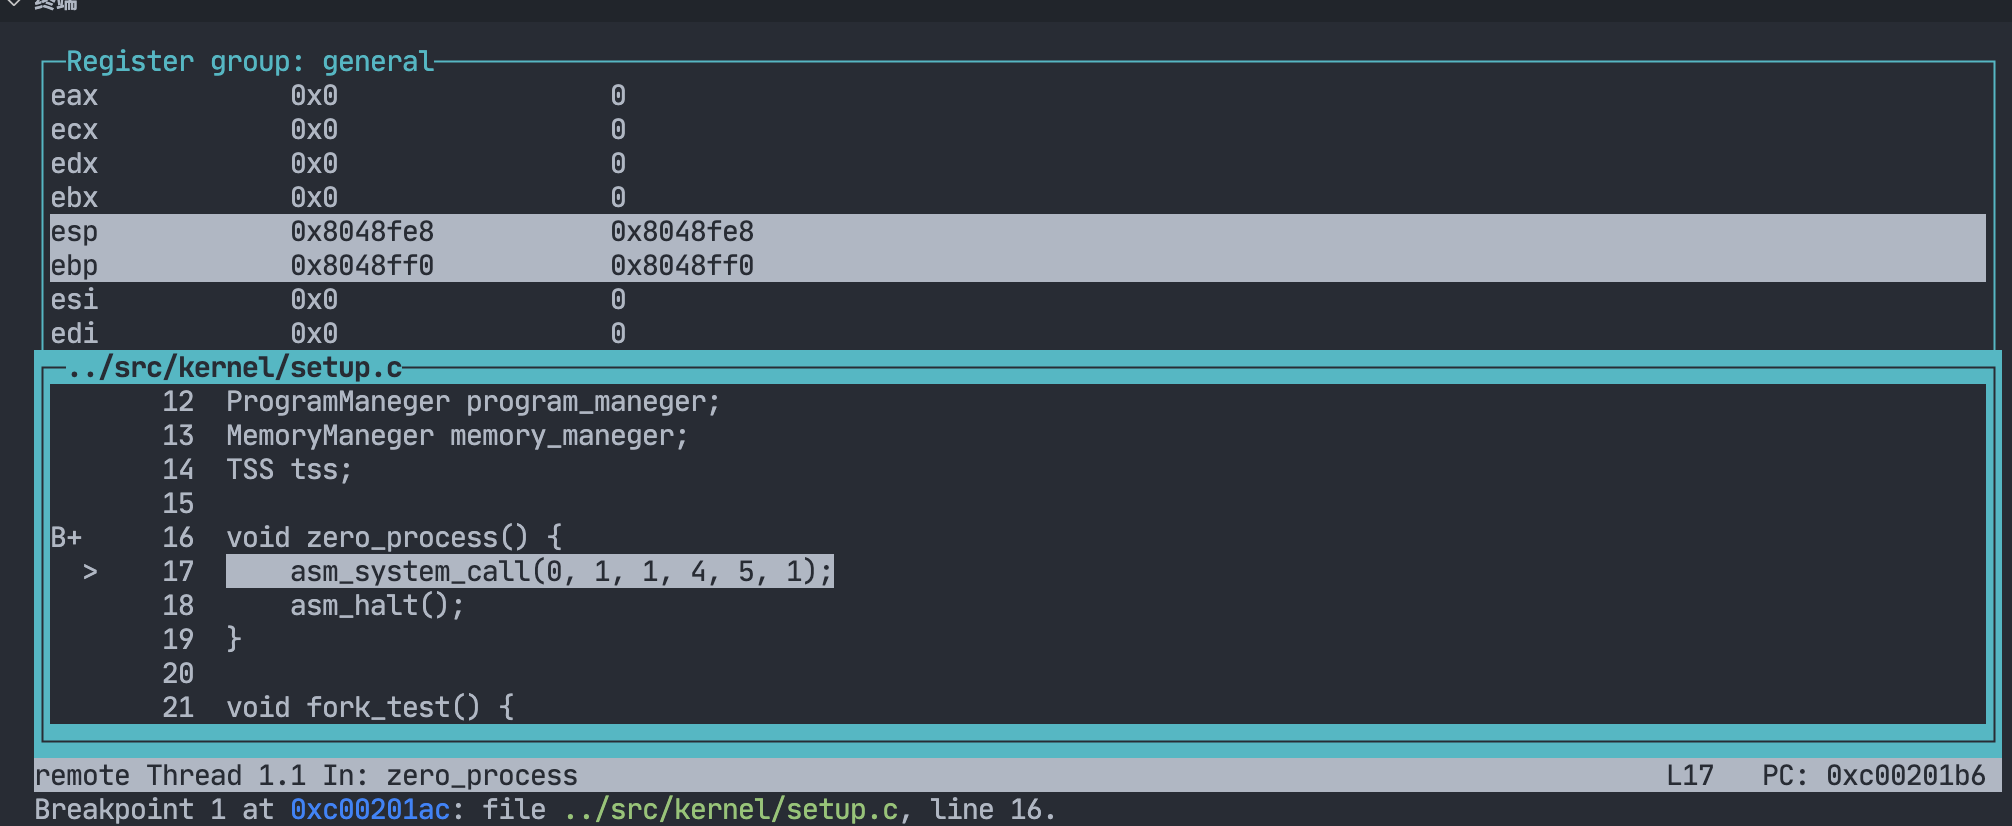
\includegraphics[width=0.6\textwidth]{figures/espStart.png}
    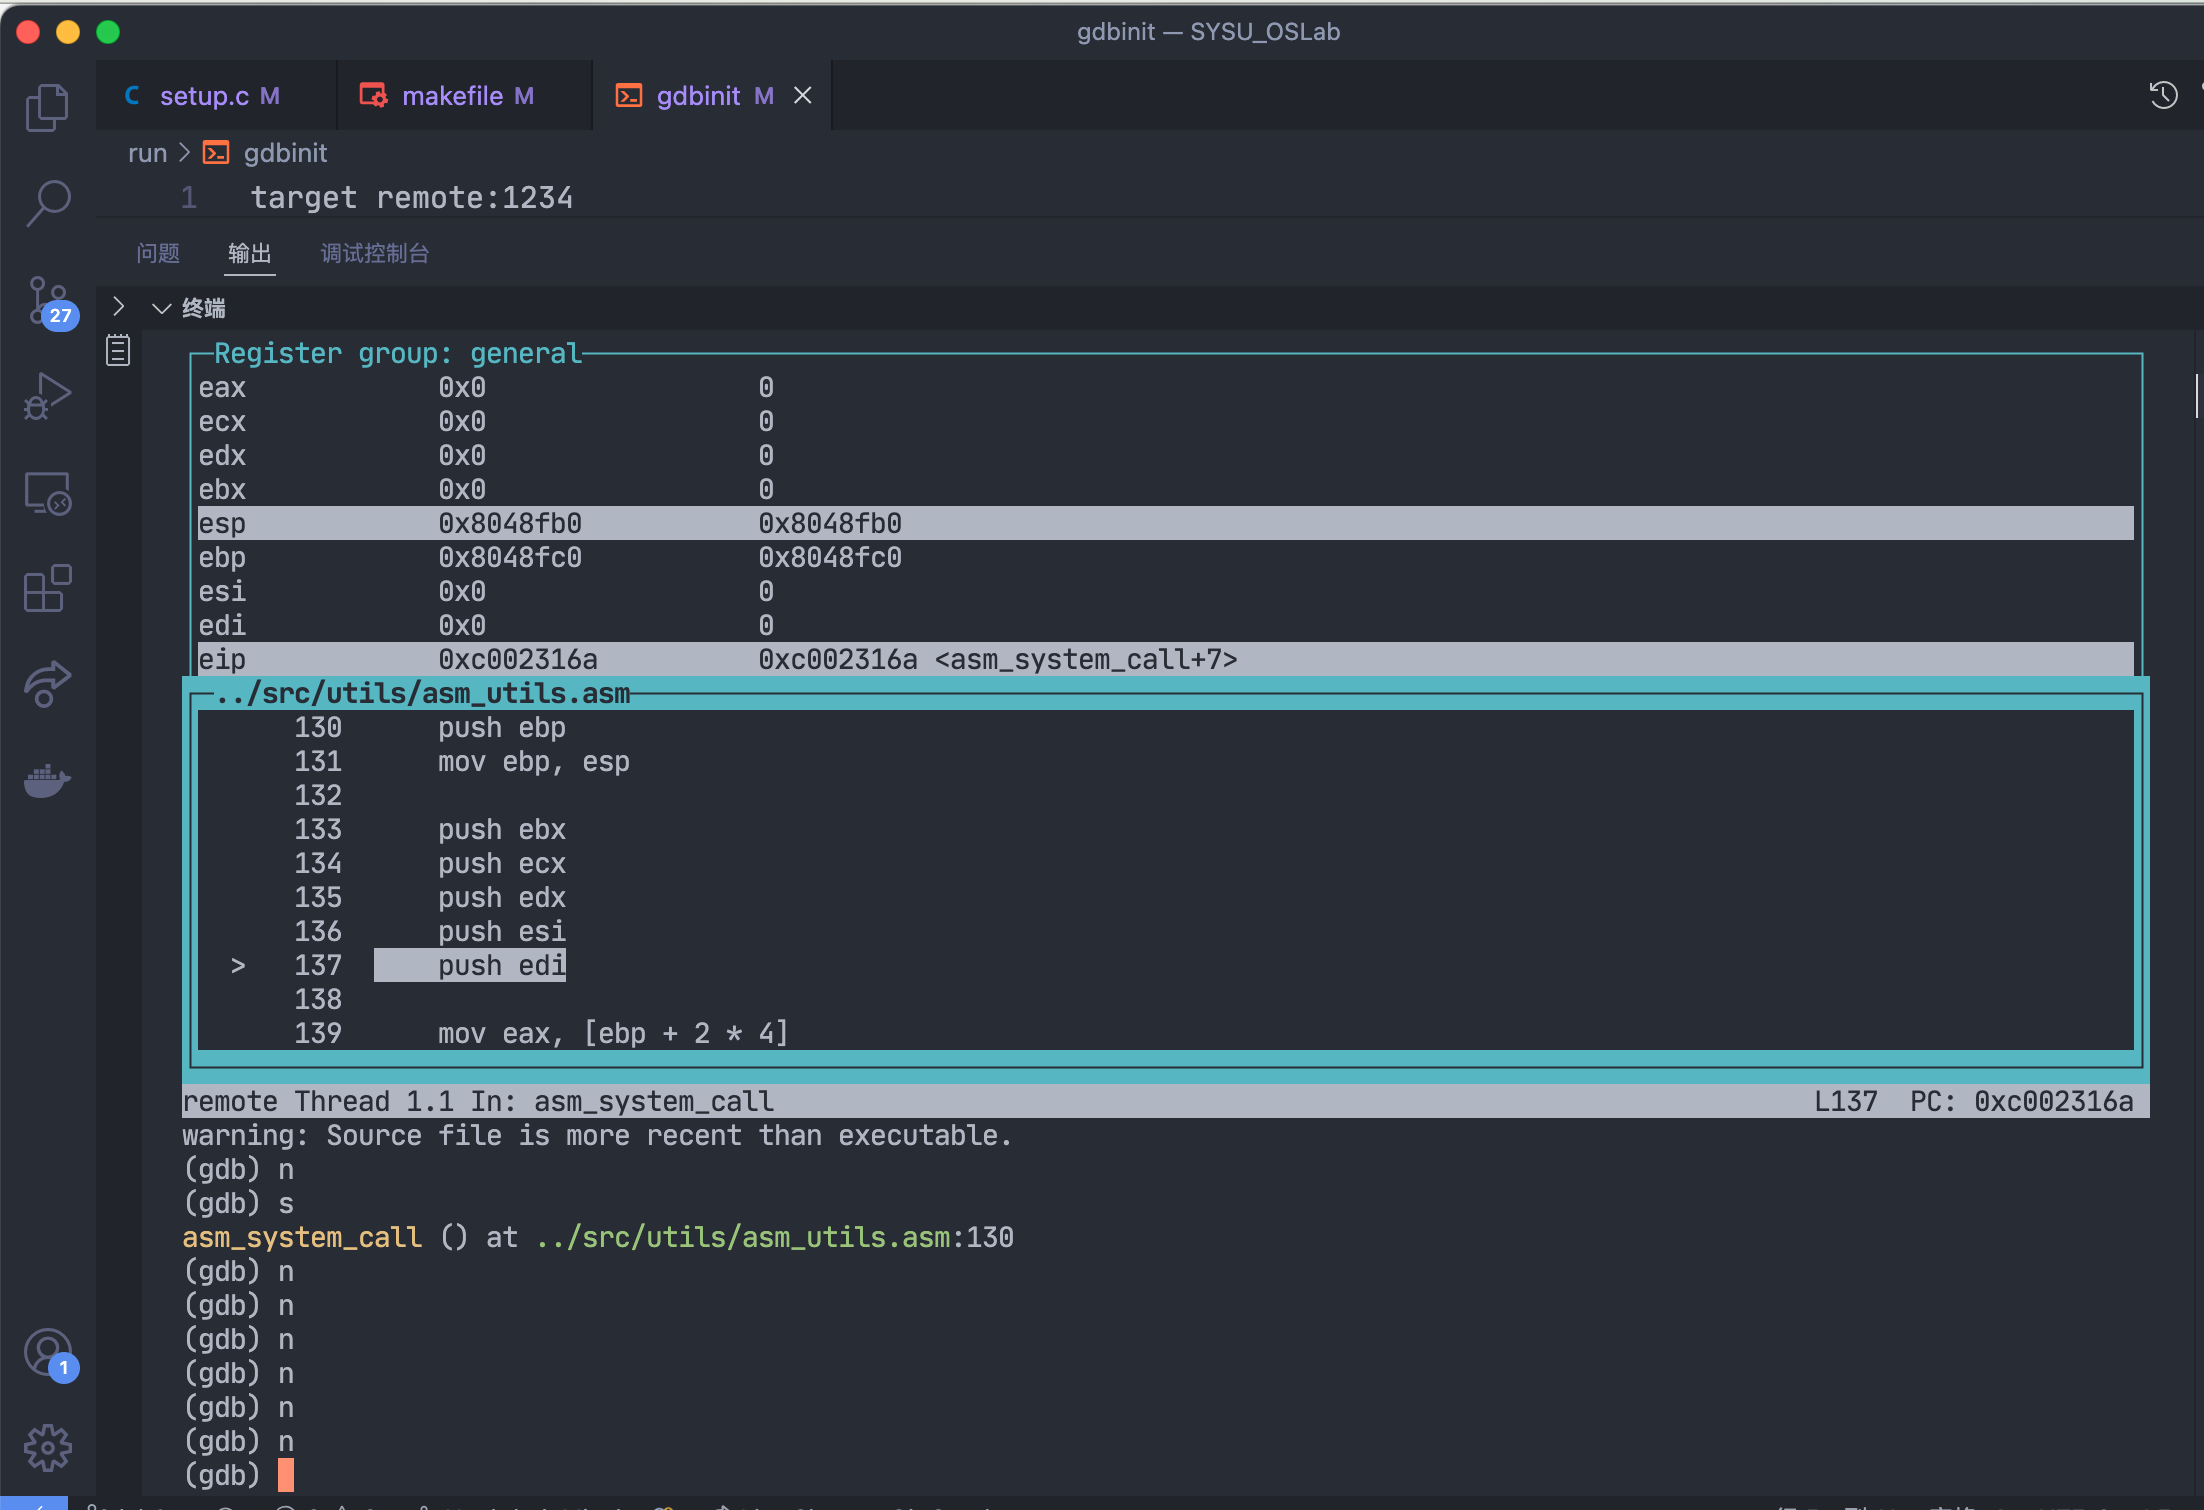
\includegraphics[width=0.6\textwidth]{figures/espMiddle.png}
    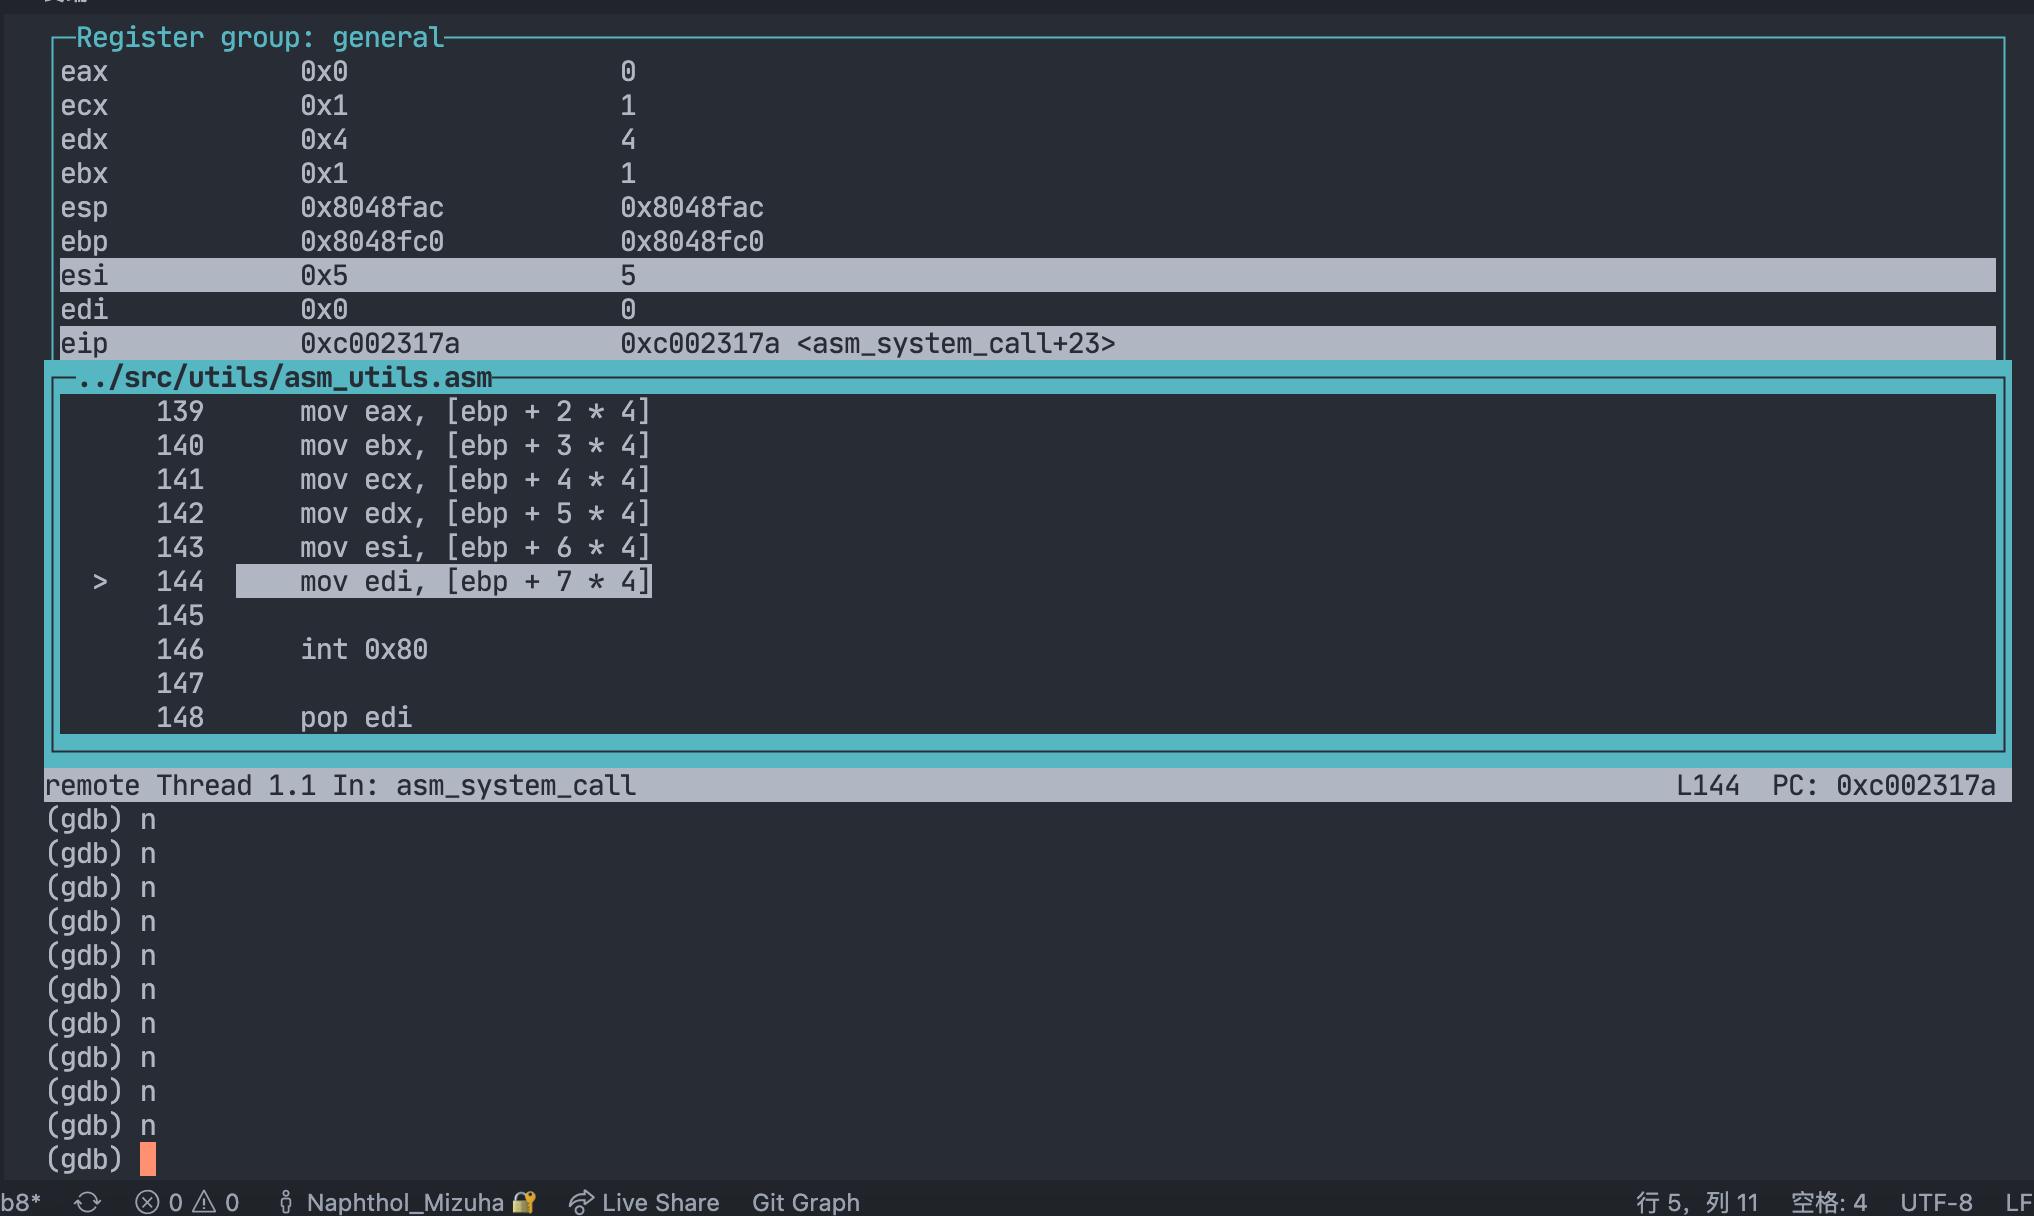
\includegraphics[width=0.6\textwidth]{figures/espMiddle2.png}
    \label{esp}
\end{figure}
\begin{figure}[H]
    \centering
    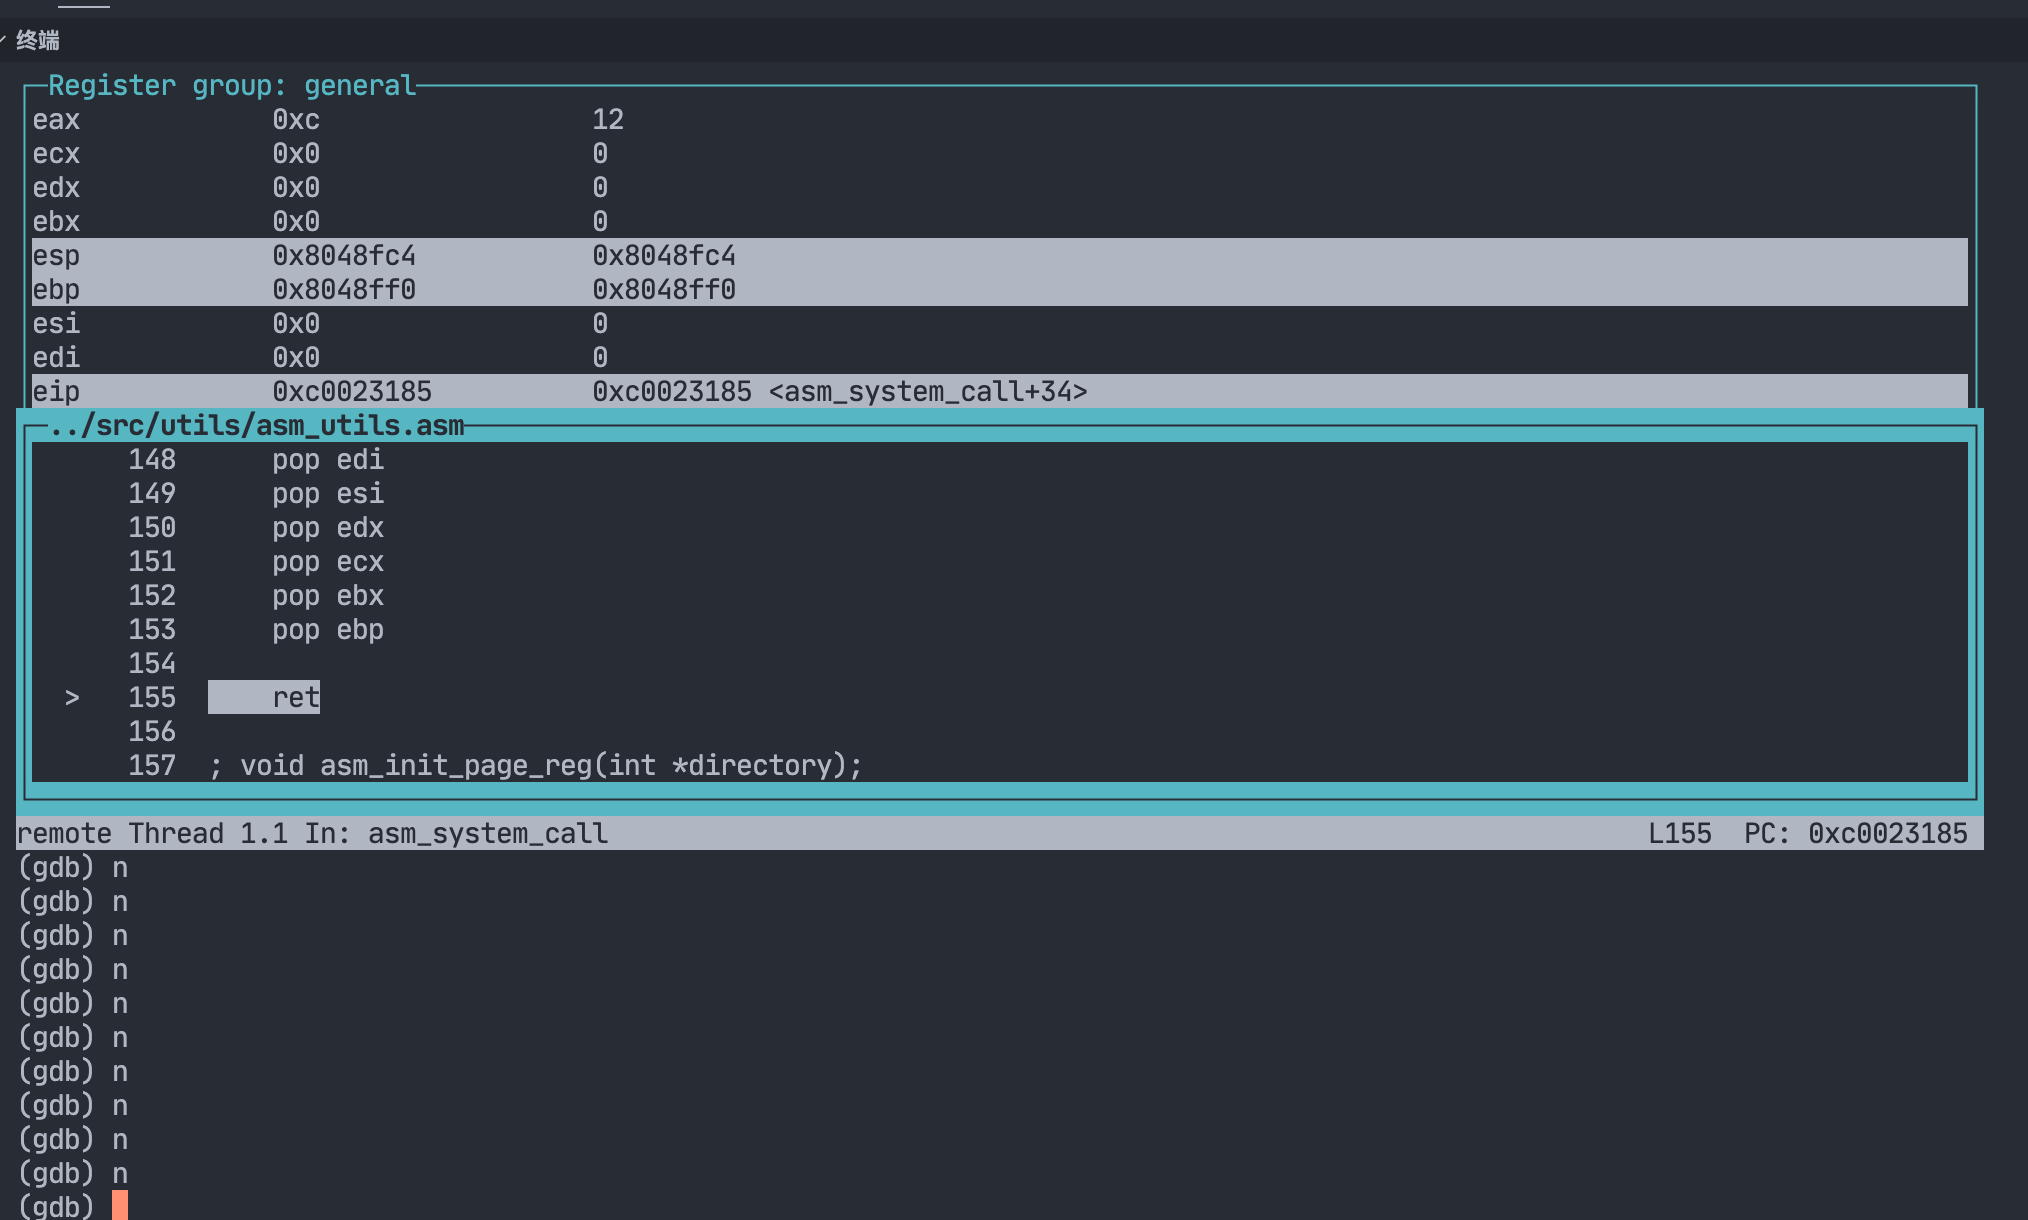
\includegraphics[width=0.6\textwidth]{figures/espEnd.png}
    \label{esp2}
\end{figure}

\subsection{根据gdb来说明TSS在系统调用执行过程中的作用}

先找到一个发起了系统调用的用户级进程,并查看TSS保存的系统级栈地址。

\begin{figure}[H]
    \centering
    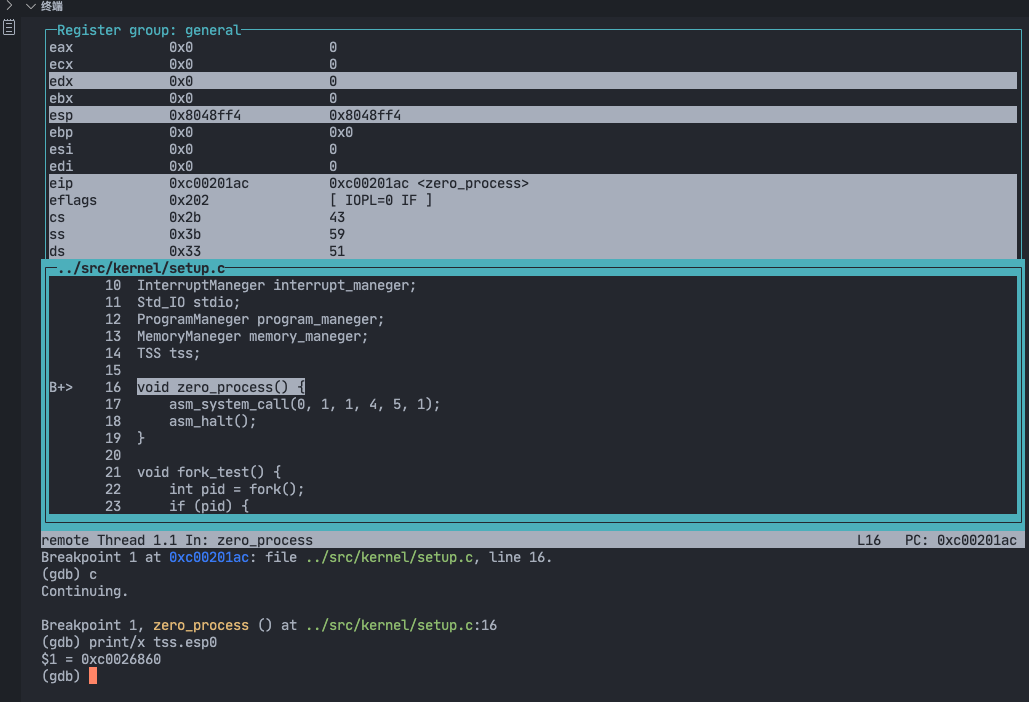
\includegraphics[width=0.6\textwidth]{figures/tss0.png}
    \label{tss0}
\end{figure}

可以看到\texttt{tss.esp0 = 0xc0026860}。然后跟踪到特权级切换的中断的指令。

\begin{figure}[H]
    \centering
    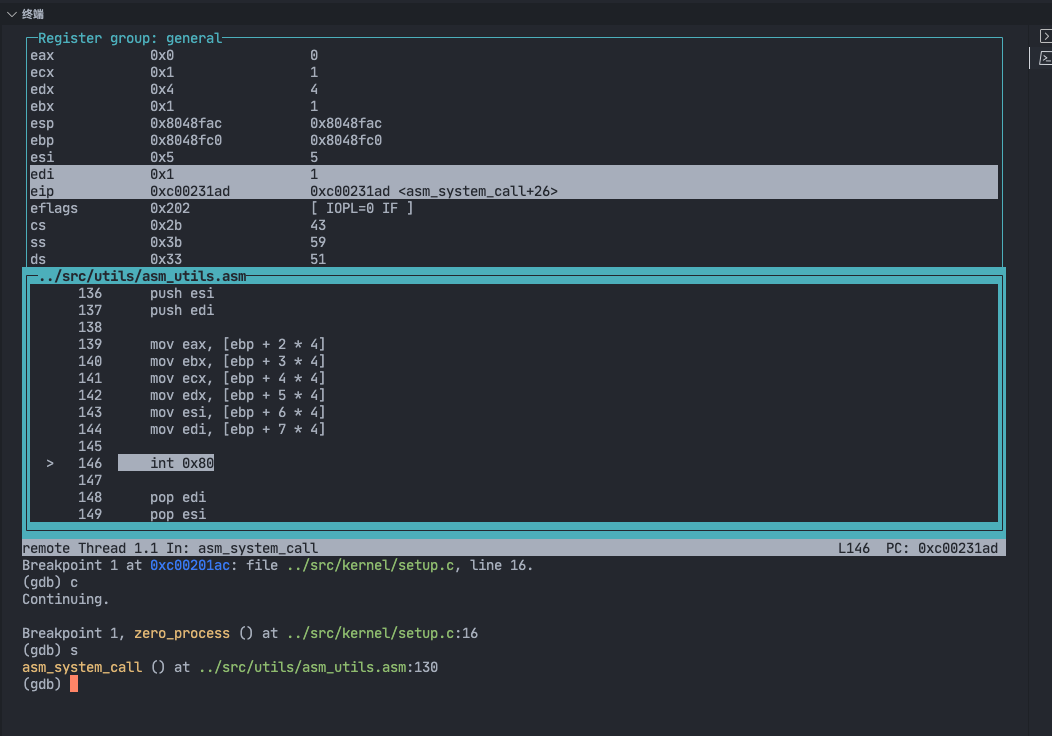
\includegraphics[width=0.6\textwidth]{figures/tss1.png}
    \vspace{1em}
    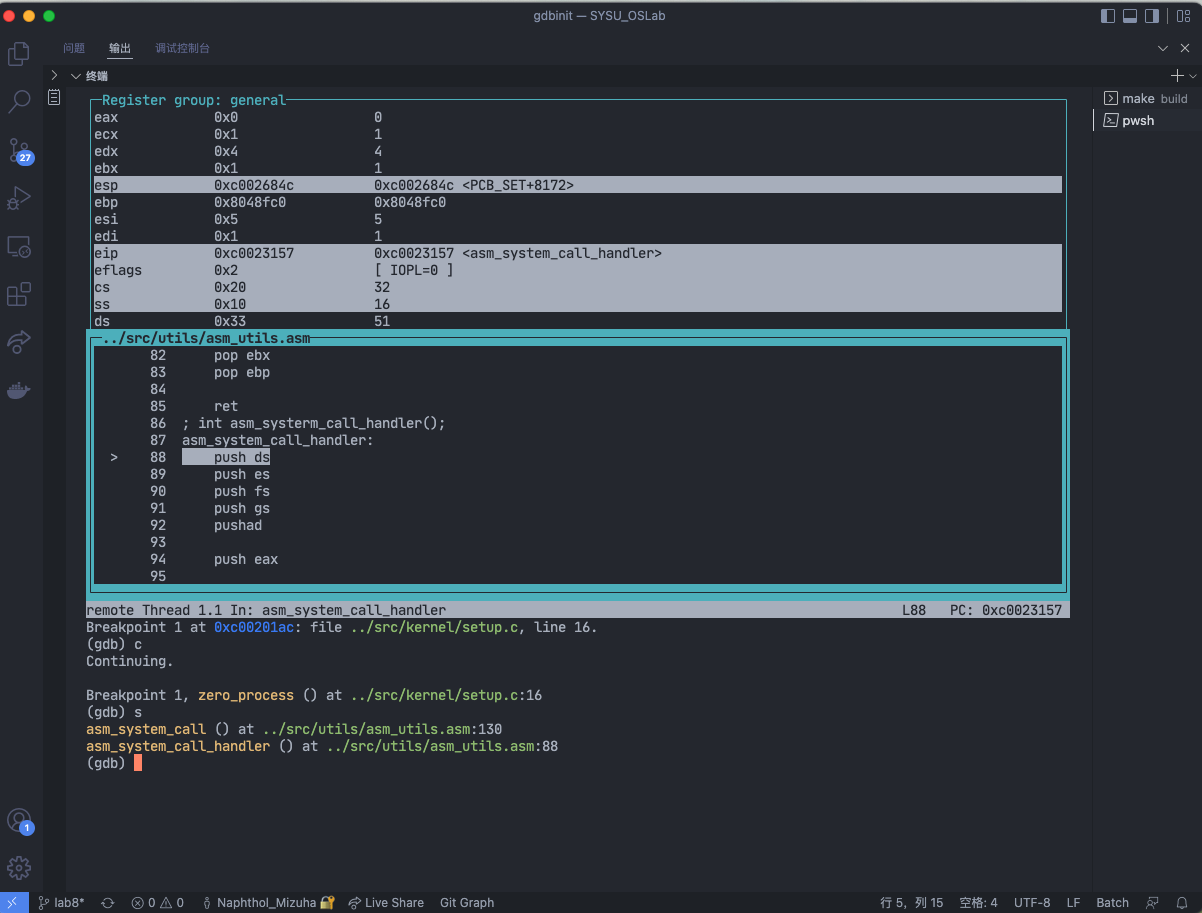
\includegraphics[width=0.6\textwidth]{figures/tss2.png}
    \label{tss1}
\end{figure}

可以看到特权级切换之后栈地址\texttt{esp}变成了\texttt{0xc002684c},
与\texttt{tss.esp0}相差了5个字节(恰好是CPU自动弹出的\texttt{ss, esp, eflags, cs, eip})。
因此,TSS的作用就是保存高特权级栈顶地址。

\subsection{从子进程第一次被调度执行时开始,逐步跟踪子进程的执行流程一直到子进程从\texttt{fork()}返回,根据gdb来分析子进程的跳转地址、数据寄存器和段寄存器的变化。同时,比较上述过程和父进程执行完\texttt{ProgramManager::fork()}后的返回过程的异同}

\subsection{根据代码逻辑和gdb来解释\texttt{fork()}是如何保证子进程的\texttt{fork()}返回值是0,而父进程的\texttt{fork()}返回值是子进程的pid}

\texttt{ProgramManeger::fork()}函数的返回值是新创建的进程的pid,也就是子进程的pid。
而在子进程复制父进程的pss时代码将pss中的\texttt{eax}设置为0,也就导致了子进程的返回值
从自己的pid变成了0。

\subsection{分析进程退出后能够隐式地调用\texttt{exit()}和此时的\texttt{exit()}返回值是0的原因}

因为在加载函数\texttt{ProgramManeger::load\_process()}中将用户栈pss的第0、1
位分别设为了\texttt{exit()}的地址以及0。这样CPU就会认为这个进程返回时需要调用
\texttt{exit()}且其参数为0。

\subsection{回收僵尸进程}